\chapter{Results}
\label{cap:cap4}

% (aproximativ 7 pagini)

% \begin{itemize}
%     \item Punerea în funcțiune/lansarea aplicației,elemente de configurare sau instalare;
%     \item Testarea sistemului (hardware/software);
%     \item Aspecte legate de încărcarea procesorului, memoriei, limitări în ce privește transmisia datelor/comunicarea;
%     \item Se prezintă datele de test/metrici/benchmarks
%     \item Aspecte legate de fiabilitate/securitate/scalabilitate;
%     \item Rezultate experimentale (grafice, tabele, etc.);
%     \item Utilizarea sistemului. 
% \end{itemize}

% \section{Nivel 1}
% \label{cap:cap4:nivel1}
%   (Figura \ref{fig:clone_trooper})

% \begin{figure}[H]
%     \centering
%     
\includegraphics[width=0.3\textwidth]{continut/capitol4/figuri/clone_trooper.png}
%     \caption{Clone Trooper\protect\footnotemark}
%     \label{fig:clone_trooper}
% \end{figure}
% \footnotetext{imagine preluată de pe un site web care nu „merită” trecut la bibliografie \url{https://www.pngitem.com/}}

% Tabelul \ref{tabel:tab_simplu} prezintă un exemplu foarte simplu de tabel în \LaTeX. Un alt exemplu este prezentat în Tabelul \ref{tabel:2} din \ref{anexa3:func_xyz}.

% \begin{table}[ht]
%     \centering
%     \caption{Exemplu de tabel simplu}
%     \label{tabel:tab_simplu}
%     \begin{tabular}{||c l c r||} 
%         \hline
%         \textbf{Col1} & \textbf{Col2} & \textbf{Col3} & \textbf{Col4} \\
%         \hline\hline
%         1 & 6 & 87837 & 787 \\ 
%         2 & 7 & 78 & 5415 \\
%         3 & 545 & 778 & 7507 \\
%         4 & 545 & 18744 & 7560 \\
%         5 & 88 & 788 & 6344 \\
%         \hline
%     \end{tabular}
% \end{table}

% \subsection{Nivel 2}
% \label{cap:cap4:nivel1:nivel2}

% \subsubsection{Nivel 3}
% \label{cap:cap4:nivel1:nivel2:nivel3}

This chapter presents the experimental results obtained from the proposed validation framework. The analysis focuses on three main aspects:

\begin{enumerate}
    \item the relationship between locally estimated performance and hidden-test performance;
    \item the effect of model complexity on validation optimism;
    \item the behavior of different biomass components under temporal and spatiotemporal validation constraints.
\end{enumerate}

The chapter begins by describing the experimental setup and evaluation procedure. It then compares the main validation protocols, analyzes per-target performance, investigates temporal generalization using Leave-One-Period-Out, and discusses the reliability and computational characteristics of the evaluation.

\section{Experimental Setup and Evaluation Procedure}

All experiments were performed using the pipeline described in Chapter~3. The public CSIRO Image2Biomass dataset was used for training and local validation. The hidden test set was used only for final scoring through the Kaggle platform.

The following experimental conditions were kept constant across all protocols:

\begin{itemize}
    \item image preprocessing and augmentation strategy;
    \item DINOv3 ViT-L/16 frozen feature extractor;
    \item $2048$-dimensional input representation;
    \item Ridge and MLP regression models;
    \item AdamW optimizer configuration for the MLP;
    \item weighted mean squared error loss;
    \item five-fold cross-validation;
    \item stratification by five intervals of \textit{Dry\_Total};
    \item five random seeds per protocol.
\end{itemize}

Each validation protocol therefore produced $25$ local runs, corresponding to $5$ folds $\times$ $5$ seeds. The local performance values reported in this chapter are expressed as mean $\pm$ standard deviation over these runs.

For the hidden-test evaluation, the optimal stopping epoch for the MLP was selected as the median of the best epochs across the $25$ runs. The final MLP model was then retrained from scratch on the entire public dataset using the protocol-specific stopping epoch. During inference, test-time augmentation with five variants was applied. For the Ridge model, a single deterministic submission was generated because the final model is deterministic after hyperparameter selection and inference. For the MLP, one submission per seed was generated, and the hidden score is reported as the mean over seeds.

The hidden test set was never inspected during model development, early stopping, or hyperparameter selection. The only information obtained from Kaggle was the final weighted $R^2_w$ score.

\section{Comparison of the main validation protocols}

Table \ref{tab:main_protocols} presents the results obtained for the three validation protocols, for both the MLP model and the Ridge model.

\begin{table}[t]
\centering
\caption{Local validation $R^2_w$, hidden-test $R^2_w$, and optimism gap for final models.}
\label{tab:main_protocols}
\footnotesize
\begin{threeparttable}
\begin{tabular}{llccc} \hline Model & Protocol & Local $R^2_w$ $\uparrow$ & Hidden $R^2_w$ $\uparrow$ & $\Delta_{\text{hidden}}$ $\downarrow$ \\ \hline
\multirow{3}{*}{MLP} 
& Random CV      & 0.841 $\pm$ 0.007 & 0.607 $\pm$ 0.013 & 0.234 \\
& Date CV        & 0.787 $\pm$ 0.007 & 0.603 $\pm$ 0.015 & 0.184 \\
& Date-State CV  & 0.794 $\pm$ 0.012 & 0.593 $\pm$ 0.018 & 0.201 \\
\hline
\multirow{3}{*}{Ridge} 
& Random CV      & 0.815 $\pm$ 0.009 & 0.561$^\dagger$ & 0.254 \\
& Date CV        & 0.735 $\pm$ 0.008 & 0.561$^\dagger$ & 0.174 \\
& Date-State CV  & 0.749 $\pm$ 0.019 & 0.561$^\dagger$ & 0.188 \\
\hline
\end{tabular}
\begin{tablenotes}
\small
\item All $\pm$ values denote sample std over seeds/folds (see text).
\item $^\dagger$ Single Kaggle submission (deterministic model); no std available.
The hidden-test score was recomputed after correcting an inference issue. An earlier conference-paper version reported 0.543 because test-time augmentation was inadvertently applied to the Ridge model, although the model was trained exclusively on non-augmented embeddings. The corrected score is 0.561.
\item The MLP stopping epoch (median over 25 runs): 35 (Random), 29 (Date), 20 (Date‑State).
\item $\uparrow$ indicates higher is better; $\downarrow$ indicates lower is better.
\end{tablenotes}
\end{threeparttable}
\end{table}

\begin{figure}[t]
    \centering
    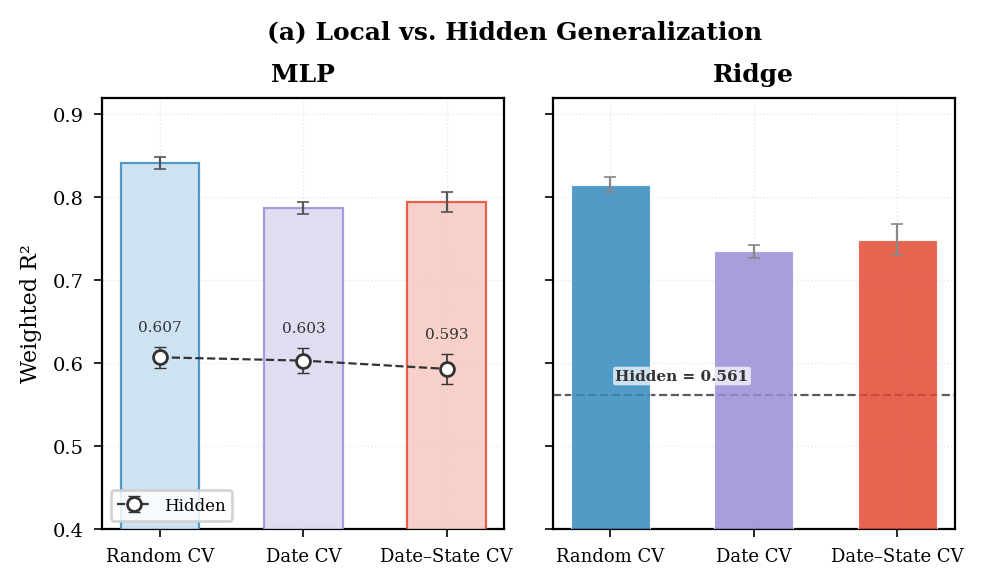
\includegraphics[width=0.8\textwidth]{continut/capitol4/figuri/fig_main_protocols.png}
    \caption{Local validation $R^2_w$ and hidden-test $R^2_w$ for the MLP and Ridge models under Random CV, Date CV, and Date-State CV. Error bars denote the standard deviation over 25 local runs for the MLP and the reported local runs for Ridge; the Ridge hidden score is deterministic.}
    \label{fig:main_protocols}
\end{figure}

Several observations emerge from Table~\ref{tab:main_protocols}.

First, the locally estimated performance is highest under Random CV for both models. The Date CV and Date-State CV protocols produce more conservative local scores. This is expected because grouped protocols reduce the amount of leakage between training and validation folds.

Second, the hidden-test scores are consistently lower than the local scores for every protocol. This confirms that the public 2015 data are not fully representative of the hidden test set. The hidden evaluation contains data from different collection periods and therefore introduces a distribution shift that is not fully captured by local validation.

Third, the optimism gap is largest under Random CV and smallest under Date CV. For the MLP, the gap decreases from 0.234 under Random CV to 0.184 under Date CV, corresponding to an approximately 21\% reduction. For Ridge, the corresponding reduction is approximately 31\%. This indicates that temporal grouping reduces the discrepancy between locally estimated and hidden-test performance. However, a noticeable gap remains under all protocols, suggesting that the distribution shift between the public and hidden data cannot be fully captured by internal validation on the 2015 dataset.

Fourth, the hidden-test scores of the MLP model are very close to each other across protocols, despite the fact that the protocols select different stopping epochs (35 for Random CV, 29 for Date CV, and 20 for Date-State CV). The differences between the hidden-test scores are within the reported standard deviations. This suggests that, once the final model is retrained on the full public dataset, the protocol-guided training duration has only a limited effect on hidden-test performance.

Figure~\ref{fig:validation_curves} shows the evolution of the local validation $R^2_w$ during MLP training for each protocol, along with the median stopping epochs reported in Table~\ref{tab:main_protocols}. The curves reflect the mean over the 25 runs, with shaded bands indicating one standard deviation.

\begin{figure}[t]
    \centering
    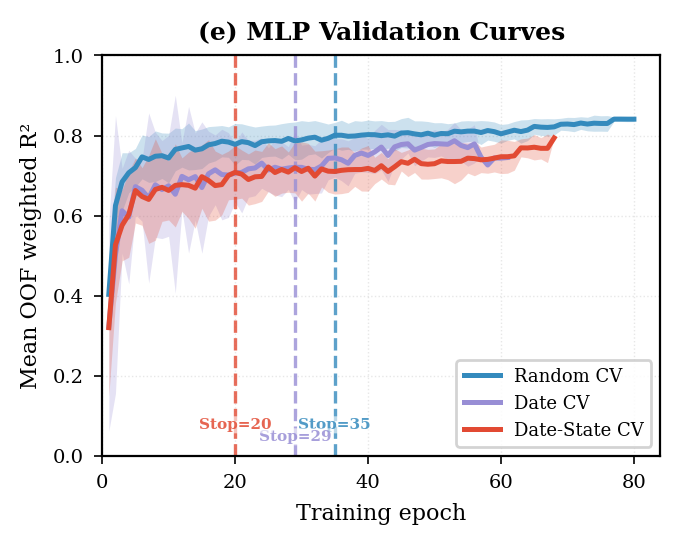
\includegraphics[width=0.8\textwidth]{continut/capitol4/figuri/fig_validation_curves.png}
    \caption{Local validation $R^2_w$ as a function of training epoch for the three validation protocols. Solid lines show the mean across 25 runs; shaded bands indicate one standard deviation. Vertical dashed lines mark the median selected stopping epoch for each protocol: 35 for Random CV, 29 for Date CV, and 20 for Date-State CV.}
    \label{fig:validation_curves}
\end{figure}

\section{Analysis of the influence of the used model} 

The similarity between the hidden-test scores obtained by the MLP and Ridge models is an important finding. 

The Ridge model contains no hidden layers, does not use dropout, and does not require early stopping. Nevertheless, it achieves a hidden-test $R^2_w$ of $0.561$, while the MLP achieves values between $0.593$ and $0.607$. The difference is at most $0.046$ in $R^2_w$. 

This result indicates that increasing the complexity of the predictor alone does not eliminate the gap between local validation and hidden-test performance. The optimism effect appears to be driven primarily by the data-splitting strategy and by distribution shifts between the public and hidden data rather than by the choice of regression model. 

One possible explanation is that the frozen DINOv3 embeddings already capture most of the predictive information available to the regression head. Once the visual representation is fixed, the remaining prediction task becomes relatively simple, and additional nonlinear transformations provide only limited improvements. This interpretation is consistent with the observation that the MLP uses different protocol-dependent stopping epochs, yet achieves very similar hidden-test scores across protocols. 

Another possible explanation is that the public dataset is relatively small and homogeneous, limiting the practical benefits of more expressive models. Under these conditions, additional model complexity may increase optimization flexibility without substantially improving generalization. 

From a methodological perspective, this finding supports the decision to use a frozen feature extractor. It isolates the validation effect from representation learning and prevents differences in backbone fine-tuning from confounding the results. Although different feature extractors would likely change the absolute performance values, the consistency of the observed trends across both MLP and Ridge suggests that the influence of the validation protocol is not specific to a single regression model.

\section{Comparison between Date CV and Date-State CV}

Date CV and Date-State CV produce similar local and hidden-test scores, with small differences that are within the observed run-to-run variability.

The Date CV protocol achieves a slightly higher hidden-test score for the MLP model ($0.603$ vs.\ $0.593$) and the same hidden-test score for the Ridge model ($0.561$). Locally, Date-State CV tends to produce slightly higher scores than Date CV, but the standard deviations overlap.

This result may appear counterintuitive. Date-State CV imposes additional grouping constraints and should, in principle, provide a more realistic estimate of performance. However, the observed differences are small and likely influenced by the following factors:

\begin{itemize}
    \item the public dataset is small, with only $357$ images;
    \item the Date-State groups are smaller and more numerous than the Date groups, which increases fold-construction variance;
    \item the hidden test set contains images from different years, while both Date CV and Date-State CV only model the internal structure of the 2015 data;
    \item the number of hidden-test evaluations is limited, and the standard deviations of the hidden scores are not negligible.
\end{itemize}

Therefore, the results should not be interpreted as evidence that Date CV is superior to Date-State CV. Instead, they suggest that after temporal grouping has been introduced, additional spatial grouping produces diminishing returns in this particular dataset.

The main limitation of both grouped protocols is that they cannot reproduce the between-year distribution shift present in the hidden test set. Since the public data come from a single year, no internal validation protocol can fully capture the difficulty of predicting biomass for images collected in other years.

\section{Per-Target Performance Analysis}

To better understand how the validation protocol affects individual biomass components, the per-target $R^2$ values were analyzed. Table~\ref{tab:per_target} presents the local per-target scores under each cross-validation protocol.

\begin{table}[t]
\centering
\footnotesize
\caption{Per-target local validation $R^2$ under each cross-validation protocol.}
\label{tab:per_target}

\begin{threeparttable}
\begin{tabular}{lccccc}
\hline
Protocol & Dry\_Green $\uparrow$ & Dry\_Dead $\uparrow$ & Dry\_Clover $\uparrow$ & GDM $\uparrow$ & Dry\_Total $\uparrow$ \\
\hline
Random CV     & 0.835 $\pm$ 0.014 & 0.570 $\pm$ 0.021 & 0.794 $\pm$ 0.023 & 0.812 $\pm$ 0.011 & 0.785 $\pm$ 0.011 \\
Date CV       & 0.736 $\pm$ 0.028 & 0.293 $\pm$ 0.159 & 0.653 $\pm$ 0.034 & 0.701 $\pm$ 0.021 & 0.742 $\pm$ 0.006 \\
Date-State CV & 0.745 $\pm$ 0.011 & 0.339 $\pm$ 0.066 & 0.664 $\pm$ 0.052 & 0.737 $\pm$ 0.012 & 0.740 $\pm$ 0.024 \\
\hline
\end{tabular}

\begin{tablenotes}
\footnotesize
\item $\uparrow$ indicates higher is better; $\downarrow$ indicates lower is better.
\end{tablenotes}
\end{threeparttable}
\end{table}

The optimism introduced by Random CV is not uniform across components.

The largest degradation after temporal grouping is observed for \textit{Dry\_Dead}. Under Random CV, the local $R^2$ is $0.570$, but it drops to $0.293$ under Date CV and to $0.339$ under Date-State CV. The standard deviation also increases substantially, from $0.021$ to $0.159$. This indicates that the prediction of dead biomass is strongly dependent on the specific conditions of each collection campaign.

\textit{Dry\_Clover} also degrades significantly, from $0.794$ under Random CV to $0.653$ under Date CV and $0.664$ under Date-State CV. This behavior is consistent with the distributional characteristics of clover biomass. Approximately $38\%$ of the plots contain no clover at all, and the coefficient of variation is very high. As a result, the relationship between visual features and clover biomass is highly heterogeneous.

In contrast, \textit{Dry\_Total} remains relatively stable across protocols. Its local $R^2$ decreases from $0.785$ under Random CV to $0.742$ under Date CV and $0.740$ under Date-State CV. The standard deviations are small in all cases. This stability is likely due to the fact that total biomass has a lower coefficient of variation and a more consistent visual signature.

\textit{Dry\_Green} and \textit{GDM} show an intermediate behavior. Their scores decrease under grouped validation but remain considerably higher than those of \textit{Dry\_Dead} and \textit{Dry\_Clover}.

These per-target results explain why the aggregated $R^2_w$ metric is only moderately sensitive to the choice of validation protocol. The weighted metric is dominated by \textit{Dry\_Total}, which is stable, while the highly affected components have smaller weights. Thus, the global score masks important differences in the generalization behavior of individual biomass components.

From a practical perspective, this analysis shows that grouped validation protocols reveal weaknesses that would otherwise remain hidden. If the goal is to deploy a model for estimating specific components such as dead biomass or clover, the use of Random CV may produce dangerously optimistic expectations.

\section{Temporal analysis using LOPO}

For a stricter evaluation of temporal generalization, the LOPO (Leave-One-Period-Out) method was also applied, in which each of the three previously defined temporal periods is used in turn as a test set.

\begin{table}[t]
\centering
\footnotesize
\caption{LOPO results using early-, middle-, and late-year calendar blocks from the 2015 public data. RMSE, MAE and Bias are reported for \textit{Dry\_Total}.}
\label{tab:lopo_summary}

\begin{threeparttable}
\begin{tabular}{lcccc} 
\hline 
Held-out period & $R^2_w \uparrow$ & RMSE $\downarrow$ & MAE $\downarrow$ & Bias $\rightarrow 0$ \\ 
\hline
Early  & 0.695 & 17.13 & 12.23 &  0.292 \\
Middle & 0.738 &  9.49 &  7.46 &  0.465 \\
Late   & 0.724 & 19.78 & 13.87 & -3.953 \\
\hline
Mean   & 0.719 & 15.46 & 11.19 & -1.065 \\
Std    & 0.024 &  4.39 &  2.75 &  2.280 \\
\hline
\end{tabular}

\begin{tablenotes} 
\footnotesize 
\item $\uparrow$ indicates higher is better, $\downarrow$ indicates lower is better, and $\rightarrow 0$ indicates values closer to zero are preferred. 
\end{tablenotes} 
\end{threeparttable}
\end{table}

In addition to $R^2_w$, RMSE and MAE, Table~\ref{tab:lopo_summary} reports the prediction bias for \textit{Dry\_Total}. Bias measures the average signed prediction error and is computed as 

\[ 
\mathrm{Bias} = \frac{1}{N} \sum_{i=1}^{N} (\hat{y}_i - y_i), 
\] 

where $\hat{y}_i$ is the predicted biomass and $y_i$ is the observed biomass. A bias of zero indicates no systematic error. Positive values indicate that the model tends to overestimate biomass on average, whereas negative values indicate systematic underestimation. Consequently, values closer to zero are preferred.

\begin{figure}[t]
    \centering
    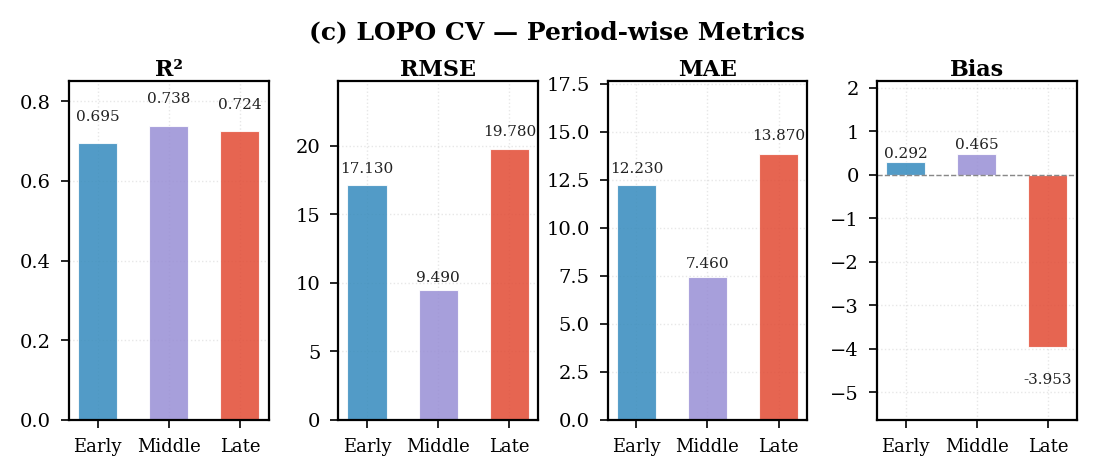
\includegraphics[width=\textwidth]{continut/capitol4/figuri/fig_lopo_summary.png}
    \caption{Leave-One-Period-Out results for the three temporal blocks of the 2015 public data. Panel (a) shows weighted $R^2_w$; panel (b) shows RMSE and MAE for \textit{Dry\_Total}; panel (c) shows the prediction bias for \textit{Dry\_Total}.}
    \label{fig:lopo_summary}
\end{figure}

The average LOPO $R^2_w$ is $0.719$, which is lower than the local scores obtained under the grouped five-fold protocols. This indicates that complete temporal separation between training and test data introduces additional difficulty that is not fully captured by standard cross-validation.

The performance is not uniform across periods. The middle period is the easiest to predict, with an $R^2_w$ of $0.738$ and the lowest RMSE and MAE values. The early period is more difficult, while the late period has the highest RMSE and MAE and the most pronounced negative bias.

The late period also contains the smallest number of images, which increases the uncertainty of the estimates. The negative bias of $-3.953$ for \textit{Dry\_Total} suggests that the model systematically underestimates total biomass in the late period. A plausible explanation is that the model is trained mainly on lower-biomass conditions from earlier periods and therefore underpredicts images associated with high biomass levels.

These observations reinforce the conclusion that temporal shifts are a significant source of generalization difficulty. Even within the same year, the relationship between visual features and biomass changes over time. Standard cross-validation, even with date-based grouping, does not fully reproduce the difficulty of predicting a completely unseen period.

\section{Reliability, Stability, and Computational Considerations}

During the preparation of the dissertation, an implementation issue was identified in the Ridge inference pipeline. The conference-paper version evaluated Ridge using test-time augmentation, despite the model being trained only on non-augmented embeddings. Re-evaluation without test-time augmentation increased the hidden-test score from 0.543 to 0.561. This correction does not change any of the qualitative conclusions of the study, including the ordering of validation protocols and the observed relationship between local and hidden-test performance.

The reliability of the experimental results is supported by several design choices.

First, each protocol was repeated with five different random seeds. This reduces the influence of stochastic variation in fold assignment, model initialization, and data augmentation. The reported standard deviations provide a measure of run-to-run variability.

Second, the hidden-test evaluation was performed without inspecting the test labels or using the test set for early stopping. The final submissions were generated using the same preprocessing and augmentation pipeline for all protocols.

Third, the use of two models with different complexities allows cross-checking the main conclusions. The fact that both Ridge and MLP produce the same ordering of optimism across protocols increases confidence that the results are not an artifact of a single model architecture.

However, several limitations affect the interpretation of the results.

\begin{itemize}
    \item The public dataset contains only $357$ images from a single year. The statistical power of the analysis is limited.
    \item The hidden test set does not provide labels or metadata. Therefore, the exact causes of the distribution shift cannot be investigated in detail.
    \item The number of hidden-test evaluations is limited by the submission mechanism. For the MLP, the hidden standard deviations are based on a small number of seeds and should not be interpreted as precise confidence intervals.
    \item The Ridge model was evaluated only once on the hidden set because it is deterministic after hyperparameter selection. Therefore, its hidden-score variance is unknown.
    \item The LOPO analysis uses small temporal blocks, especially the late period, which contains only $96$ images.
\end{itemize}

From a computational perspective, the proposed pipeline is efficient. All experiments were performed on a laptop equipped with an Intel Core i5-11300H processor, 16~GB of RAM, and an NVIDIA GeForce RTX~3050 Laptop GPU with 4~GB of VRAM. 

The DINOv3 embeddings are precomputed once and reused for all experiments. During embedding extraction, automatic mixed precision (AMP) with the \texttt{bfloat16} data type is used whenever supported. Since the backbone operates in frozen mode, gradient computation is disabled and only forward passes are required. This reduces both memory consumption and execution time while preserving the quality of the resulting embeddings. 

The use of a frozen DINOv3 backbone substantially reduces the computational requirements compared with end-to-end fine-tuning. Feature extraction is performed only once, after which all validation protocols and regression models operate exclusively on precomputed 2048-dimensional embeddings. Consequently, repeated cross-validation experiments require only the training of lightweight regression models rather than repeated optimization of the full ViT-L/16 architecture. 

The main computational cost is the initial extraction of augmented embeddings. However, this cost is incurred only once and the resulting embeddings are stored on disk for reuse throughout all experiments. The MLP training stage is lightweight because it operates exclusively on fixed embeddings, while the Ridge baseline requires only linear regression with a small hyperparameter search over seven regularization values. 

The pipeline is also modular. The data-loading, preprocessing, feature-extraction, model-training, validation, and evaluation components are implemented as separate modules. This makes it possible to add new validation protocols or prediction models without modifying the rest of the system.

\section{Summary of Experimental Findings} 

The experimental results support the following conclusions. 
\begin{itemize} 
\item Random CV produces the highest local validation scores but also the largest optimism gap. This suggests that part of the apparent performance gain is explained by temporal and spatial similarities between training and validation samples. 

\item Date-based grouping reduces the optimism gap relative to Random CV. For the MLP model, the gap decreases from $0.234$ to $0.184$, corresponding to an approximately $21\%$ reduction. For the Ridge model, the gap decreases from $0.254$ to $0.174$, corresponding to an approximately $32\%$ reduction. This indicates that temporal grouping provides a more realistic estimate of generalization performance. However, a noticeable discrepancy between local and hidden-test performance remains. 

\item Date-State CV does not provide a clear improvement over Date CV in hidden-test performance. While it introduces a stricter grouping strategy, the observed gains are small and inconsistent across models. 

\item The validation protocol has a much larger effect on the locally estimated performance than on the final hidden-test performance. Although the local $R^2_w$ values differ substantially between protocols, the hidden-test scores are very similar. This suggests that the primary effect of the protocol is to change the reliability of the performance estimate rather than the quality of the final model. 

\item Model complexity has only a limited effect on hidden-test performance when the visual representation is fixed. Despite the large difference in complexity between Ridge and MLP, both models exhibit similar patterns of optimism and achieve comparable hidden-test scores. 

\item Per-target analysis reveals that biomass components are affected differently by temporal validation constraints. In particular, \textit{Dry\_Dead} and \textit{Dry\_Clover} experience considerably larger performance degradations under grouped validation than \textit{Dry\_Total}. 

\item LOPO analysis shows that temporal generalization is more difficult than suggested by standard cross-validation. Performance varies across temporal periods, and the late-period split exhibits a systematic tendency to underestimate total biomass. 

\item The hidden test set contains distribution shifts that cannot be fully reproduced by any internal validation protocol based solely on the 2015 public data. Consequently, even the grouped protocols cannot perfectly predict the performance that will be achieved on truly unseen data. 
\end{itemize} 

These findings have direct implications for model evaluation in agricultural machine learning. They show that the choice of validation protocol can be as important as the choice of model architecture when estimating real-world performance. In the present study, grouped validation protocols do not substantially improve the final hidden-test score, but they do provide more conservative and more reliable estimates of model generalization. This distinction is important because an accurate estimate of future performance is often more valuable than a small increase in local validation accuracy.

% În această etapă sunt evaluate cele trei protocoale de validare prezentate în capitolul anterior. Analiza urmărește atât performanța estimată local prin validare încrucișată, cât și performanța obținută pe setul de test ascuns al competiției Kaggle.

% În prima parte este realizată o comparație între protocoalele Random Cross-Validation, Date Cross-Validation și Date-State Cross-Validation din perspectiva metricii $R^2_w$, a epocii de oprire selectate și a performanței obținute pe setul de test ascuns. Ulterior, sunt analizate rezultatele pentru fiecare componentă a biomasei și este realizată o evaluare suplimentară folosind strategia LOPO (Leave-One-Period-Out), pentru a investiga mai detaliat diferența dintre performanța estimată local și capacitatea reală de generalizare.

% \section{Compararea principalelor protocoale de validare}

% Tabelul \ref{tab:main_protocols} prezintă rezultatele obținute pentru cele trei protocoale de validare, atât pentru modelul MLP, cât și pentru modelul Ridge.

% Rezultatele evidențiază un comportament consistent pentru ambele modele. Protocolul Random CV obține cele mai mari valori ale metricii locale \(R^2_w\), în timp ce protocoalele bazate pe grupare temporală produc estimări mai conservatoare. În toate cazurile, performanța măsurată pe setul de test ascuns este semnificativ mai redusă decât performanța estimată local.

% Această diferență se reflectă direct în valorile optimism gap-ului, unde valorile mai mari indică o supraestimare mai accentuată a performanței reale. Concordanța rezultatelor observate pentru două modele cu complexități foarte diferite sugerează că optimismul excesiv nu este cauzat în principal de arhitectura modelului, ci de modul în care sunt împărțite datele în procesul de validare.

% \begin{table}[t]
% \centering
% \caption{Local validation $R^2_w$, hidden-test $R^2_w$, and optimism gap for final models.}
% \label{tab:main_protocols}
% \begin{threeparttable}
% \resizebox{\columnwidth}{!}{%
% \begin{tabular}{llccc}
% \hline
% Model & Protocol & Local $R^2_w$ & Hidden $R^2_w$ & $\Delta_{\text{hidden}}$ \\
% \hline
% \multirow{3}{*}{MLP} 
% & Random CV      & 0.841 $\pm$ 0.007 & 0.607 $\pm$ 0.013 & 0.234 \\
% & Date CV        & 0.787 $\pm$ 0.007 & 0.603 $\pm$ 0.015 & 0.184 \\
% & Date-State CV  & 0.794 $\pm$ 0.012 & 0.593 $\pm$ 0.018 & 0.201 \\
% \hline
% \multirow{3}{*}{Ridge} 
% & Random CV      & 0.815 $\pm$ 0.009 & 0.543$^\dagger$ & 0.272 \\
% & Date CV        & 0.735 $\pm$ 0.008 & 0.543$^\dagger$ & 0.192 \\
% & Date-State CV  & 0.749 $\pm$ 0.019 & 0.543$^\dagger$ & 0.206 \\
% \hline
% \end{tabular}
% }
% \begin{tablenotes}
% \small
% \item All $\pm$ values denote sample std over seeds/folds (see text).
% \item $^\dagger$ Single Kaggle submission (deterministic model); no std available.
% \item The MLP stopping epoch (median over 25 runs): 35 (Random), 29 (Date), 20 (Date‑State).
% \end{tablenotes}
% \end{threeparttable}
% \end{table}

% Pentru modelul MLP se observă că cele trei scoruri obținute pe setul ascuns sunt foarte apropiate între ele și se încadrează în intervalele determinate de deviațiile standard raportate. Acest lucru este valabil în ciuda faptului că fiecare protocol conduce la o epocă optimă diferită pentru oprirea antrenării. În consecință, utilizarea unui mecanism de early stopping specific protocolului nu pare să influențeze semnificativ performanța finală de generalizare.

% Aceste observații evidențiază importanța designului protocolului de validare atunci când se urmărește obținerea unor estimări realiste ale performanței în condiții de utilizare reală.

% \subsection{Analiza influenței modelului utilizat}

% Similaritatea scorurilor obținute pe setul ascuns pentru modele antrenate cu un număr diferit de epoci sugerează faptul că rețeaua MLP converge rapid atunci când utilizează embedding-uri DINOv3 fixe.

% Această interpretare este susținută și de rezultatele modelului Ridge. Deși acesta nu conține straturi ascunse și nu utilizează mecanisme de early stopping, obține un scor \(R^2_w\) de 0.543 pe setul ascuns, aflându-se la mai puțin de 0.06 puncte de performanța modelului MLP.

% Diferența relativ redusă dintre cele două modele sugerează că simpla creștere a complexității predictorului nu este suficientă pentru eliminarea diferenței dintre performanța locală și cea observată pe setul de test ascuns. O explicație posibilă este că parte din această diferență este determinată de limitările reprezentării vizuale produse de backbone-ul frozen utilizat. Totuși, factori precum dimensiunea redusă a setului de date sau variabilitatea etichetelor pot contribui, de asemenea, la capacitatea limitată de generalizare.

% Deși modelul DINOv3 a fost ales exclusiv ca extractor puternic de caracteristici pentru izolarea efectului protocolului de validare, valorile absolute ale performanței pot varia atunci când sunt utilizate alte reprezentări vizuale. Cu toate acestea, efectul de optimism introdus de validare este de așteptat să rămână relevant indiferent de backbone-ul folosit.

% \subsection{Comparația dintre Date CV și Date-State CV}

% Cele două protocoale bazate pe grupare produc rezultate similare, diferențele dintre ele fiind relativ reduse.

% În mod intuitiv, s-ar putea presupune că protocolul Date-State CV, care impune constrângeri suplimentare asupra grupării, ar trebui să ofere estimări mai realiste și implicit rezultate mai bune pe setul ascuns. Totuși, în experimentele realizate, Date CV obține o valoare ușor superioară a metricii \(R^2_w\) pe setul de test ascuns (0.603 față de 0.593).

% Această inversare poate fi explicată prin suprapunerea semnificativă a intervalelor de deviație standard și prin dimensiunea redusă a setului public de date. Prin definirea unor grupuri mai mici, Date-State CV introduce o variabilitate mai mare în construirea foldurilor, ceea ce crește sensibilitatea rezultatelor la zgomotul de eșantionare.

% Având în vedere dimensiunea redusă a datasetului și numărul limitat de evaluări disponibile pe setul ascuns, aceste diferențe nu trebuie interpretate ca fiind semnificative statistic.

% Mai important, ambele protocoale modelează doar structura internă a datelor din anul 2015, în timp ce setul de test ascuns conține imagini provenite din anii 2014 și 2016. Dacă variațiile dintre ani reprezintă principala sursă de schimbare a distribuției, niciuna dintre strategiile analizate nu poate reproduce complet dificultatea întâlnită pe benchmark-ul ascuns.

% Rezultatele sugerează astfel existența unor beneficii descrescătoare ale constrângerilor suplimentare de grupare: după introducerea grupării temporale, stratificarea suplimentară în funcție de statul australian reduce doar marginal optimismul estimării.

% \section{Analiza performanței la nivelul fiecărei componente de biomasă}

% Pentru a înțelege mai bine efectul protocolului de validare asupra fiecărei componente a biomasei, au fost analizate valorile individuale ale metricii $R^2_w$ pentru fiecare variabilă țintă.

% \begin{table}[t]
% \centering
% \footnotesize
% \caption{Per-target local validation $R^2$ under each cross-validation protocol.}
% \label{tab:per_target}
% \resizebox{\columnwidth}{!}{%
% \begin{tabular}{lccccc}
% \hline
% Protocol & Dry\_Green & Dry\_Dead & Dry\_Clover & GDM & Dry\_Total \\
% \hline
% Random CV     & 0.835 $\pm$ 0.014 & 0.570 $\pm$ 0.021 & 0.794 $\pm$ 0.023 & 0.812 $\pm$ 0.011 & 0.785 $\pm$ 0.011 \\
% Date CV       & 0.736 $\pm$ 0.028 & 0.293 $\pm$ 0.159 & 0.653 $\pm$ 0.034 & 0.701 $\pm$ 0.021 & 0.742 $\pm$ 0.006 \\
% Date-State CV & 0.745 $\pm$ 0.011 & 0.339 $\pm$ 0.066 & 0.664 $\pm$ 0.052 & 0.737 $\pm$ 0.012 & 0.740 $\pm$ 0.024 \\
% \hline
% \end{tabular}
% }
% \end{table}

% Rezultatele din Tabelul \ref{tab:per_target} arată că optimismul introdus de Random Cross-Validation nu este distribuit uniform între toate componentele biomasei.

% Cea mai mare degradare a performanței după introducerea grupării temporale este observată pentru variabila \textit{Dry\_Dead}, urmată de \textit{Dry\_Clover}. În schimb, variabila \textit{Dry\_Total} rămâne relativ stabilă indiferent de protocolul utilizat.

% Această diferență poate fi explicată prin caracteristicile distribuțiilor asociate fiecărei variabile. Componentele \textit{Dry\_Dead} și \textit{Dry\_Clover} prezintă cea mai mare variabilitate, având coeficienți de variație de 1.03 și respectiv 1.82, în comparație cu 0.62 pentru \textit{Dry\_Total}. În plus, \textit{Dry\_Clover} este puternic dezechilibrată, aproximativ 38\% dintre parcele neconținând deloc trifoi.

% Deși aceste componente sunt prezente în majoritatea imaginilor, distribuțiile lor puternic asimetrice fac ca predicția să depindă într-o măsură mai mare de particularitățile fiecărei campanii de colectare. Eliminarea acestor indicii prin gruparea temporală determină o scădere semnificativă a performanței.

% În contrast, \textit{Dry\_Total} prezintă o relație mai stabilă între caracteristicile vizuale și valoarea țintă, fiind considerabil mai puțin influențată de strategia de împărțire a datelor.

% Această stabilitate explică și de ce metrica agregată $R^2_w$ este mai puțin sensibilă la alegerea protocolului decât ar sugera analiza individuală a componentelor. Rezultatele indică faptul că validarea grupată reușește să evidențieze fragilități specifice anumitor componente ale biomasei, care sunt mai puțin vizibile atunci când se analizează exclusiv scorul global.

% \section{Analiza temporală utilizând LOPO}

% Pentru o evaluare mai strictă a generalizării temporale a fost aplicată și metoda LOPO (Leave-One-Period-Out), în cadrul căreia fiecare dintre cele trei perioade temporale definite anterior este utilizată pe rând ca set de test.

% \begin{table}[t]
% \centering
% \footnotesize
% \caption{LOPO results using early-, middle-, and late-year calendar blocks from the 2015 public data.}
% \label{tab:lopo_summary}
% \resizebox{\columnwidth}{!}{%
% \begin{tabular}{lccccc}
% \hline
% Held-out period & $R^2_w$ & RMSE (Dry\_Total) & MAE (Dry\_Total) & Bias (Dry\_Total) \\
% \hline
% Early  & 0.695 & 17.13 & 12.23 &  0.292 \\
% Middle & 0.738 &  9.49 &  7.46 &  0.465 \\
% Late   & 0.724 & 19.78 & 13.87 & -3.953 \\
% \hline
% Mean   & 0.719 & 15.46 & 11.19 & -1.065 \\
% Std    & 0.024 &  4.39 &  2.75 &  2.280 \\
% \hline
% \end{tabular}
% }
% \end{table}

% Rezultatele prezentate în Tabelul \ref{tab:lopo_summary} indică o valoare medie $R^2_w$ de 0.719, semnificativ mai mică decât valorile obținute prin protocoalele de validare grupate bazate pe 5 folduri.

% Acest rezultat sugerează că separarea temporală completă între datele de antrenare și cele de testare introduce dificultăți suplimentare care nu sunt surprinse integral de procedurile standard de cross-validation.

% Performanța nu este uniformă între cele trei intervale temporale analizate. Perioada de mijloc este cea mai ușor de prezis, în timp ce perioadele timpurie și târzie sunt considerabil mai dificile.

% În cazul perioadei târzii se observă cele mai mari valori RMSE și MAE pentru biomasa totală, precum și cel mai pronunțat bias negativ. Totuși, această perioadă conține și cel mai mic număr de imagini, ceea ce conduce la o incertitudine mai mare a estimărilor.

% Aceste observații sugerează că dificultatea procesului de generalizare nu este uniformă nici măcar în interiorul datelor din anul 2015. Astfel, alegerea unei anumite împărțiri temporale poate influența semnificativ performanța estimată local.

% Bias-ul negativ pronunțat observat în perioada târzie poate fi explicat prin faptul că modelul este antrenat predominant pe condiții caracterizate de valori mai mici ale biomasei și dezvoltă astfel tendința de a subestima imaginile asociate unor niveluri ridicate ale biomasei.

% Per ansamblu, analiza LOPO consolidează concluziile obținute în secțiunea anterioară. Protocoalele de validare grupate reduc efectele de scurgere a informației (data leakage), însă continuă să producă estimări optimiste ale performanței. Rezultatele sugerează că setul de test ascuns conține schimbări de distribuție care sunt doar parțial reproduse de protocoalele utilizate local. În același timp, dimensiunea redusă și distribuția dezechilibrată a blocurilor temporale impun interpretarea acestor rezultate ca observații orientative și nu ca o cuantificare exactă a capacității de generalizare temporală.